%% BEGIN Jaza/Visitor seminar, LIFC, Besancon, Nov 2001
%
% Adapted from semsamp2.ps for seminar.sty, v0.93 (and maybe later).
% This file contains both landscape and portrait mode slides.
% Choose one of the following to print them out:
%  - If using PSTricks, try the semcolor style option.
%  - If using Rokicki's dvips, try the semrot style option.
%  - To print the landscape slides, put \landscapeonly in the preamble.
%    To print the portrait slides, include the portrait style option and
%    put \portraitonly in the preamble.
%
% \begin{slide}[7.3in,5.5in] \label{questions}
% \heading{Questions}
% 
% \begin{itemize}
%   {\overlay1\item When could {\blue there be overload} in networks?}
%   \item What mechanims make the receivers and senders better off?
%   \item How does the welfare {\red of the senders} and receivers ...
% \end{itemize}
% \end{slide}
%
% \def\slidefuzz{15pt}
% \medskip


\documentclass[%
  slidesonly,%  Try notes or notesonly instead.
  %notes,%      Use instead of slidesonly to typeset the notes.
  %notesonly,%  Use instead of slidesonly to typeset notes and slides.
  %semcolor,%   Try me if using PSTricks.
  %semrot,%     Try me if using Rokicki's dvips.
  %semhelv,%    Try me if using a PostScript printer.
  %article,%    Try me.
  %portrait,%   Try me.
  sem-a4,%     Try me if using A4 paper.
  semlayer%     This must be included, but you need the semcolor option to
  ]{seminar}                                  % actually see the overlays.

\usepackage[dvips]{graphicx}
%\usepackage{pstricks}
\usepackage{multicol}
\usepackage{z-eves}
\slidesmag{4}
\articlemag{1}
\newenvironment{algo}{\tt \begin{tabbing} 123\=123\=123\=123\=123\=123\=123\=123\=123\=123\=123\=123\=\kill}{\end{tabbing}\rm}

%\twoup                     % Try me for twoup printing.

%\portraitonly              % To print only portrait slides
%\landscapeonly             % To print only landscape slides

%\notslides{\ref{questions}-7,1}   %Try me: The slides are omitted.
%\onlyslides{\ref{questions}-7,1}  %Try me: Only these slides are included.
%\onlynotestoo                     %Try me: For selecting notes as well.

\colorlayers{red,blue}      % Try deleting this if using the semcolor option,
                            % to get \blue and \red to use PostScript color.

%\overlaysfalse             % Suppress overlays with semcolor option.
%\layersfalse               % Suppress color layers with semcolor option.

\rotateheaderstrue          % Try this out if using rotation macros.


\title{BZ-TT: Integrating Z}
\author{Dr Mark Utting, Waikato University, NZ\\
        LIFC Professeur Invit\'{e}: Juillet 2001 - Janvier 2002}
\date{7 Dec 2001}

\newcommand{\sref}[1]{SLIDE \ref{#1}}
\newcommand{\heading}[1]{\begin{center}\large\bf #1\end{center}}

\newenvironment{machine}[1]{
    \begin{tabular}{@{\qquad}l}\textbf{\kern-1em machine}\ #1\\ }{
    \\ \textbf{\kern-1em end} \end{tabular} }
\newcommand{\machineInit}{\\ \textbf{\kern-1em init} \\}
\newcommand{\machineOps}{\\ \textbf{\kern-1em ops} \\}

\newpagestyle{MH}%
  {BZ-TT: B/Z Testing Tools \hfil\thepage}{}
\pagestyle{MH}

\begin{document}

\maketitle          % This won't show up when \onlynotestoo is in effect.

\begin{slide}
  \ifslidesonly              % Title slide only for slidesonly selection.
    \maketitle
    \addtocounter{slide}{-1}
    \slidepagestyle{empty}
  \fi
  \medskip
  \begin{enumerate}
    \item Z and B: Similarities and Differences
    \item Machines in Z?
    \item Design of Z to B translator.
    \item Z-specific difficulties.
  \end{enumerate}
\end{slide}


\begin{slide}\label{history}%
\begin{tabular}{lll}
Z & = & sets+relns+funcs+seqs+bags + schema-calculus \\
\hline
  && Developed at Oxford in the 1980s (Abrial+others). \\
  && Developed with extensive industry collaboration. \\
  && Widely known, used and taught. \\
  && Is a draft ISO standard. \\[1ex]
B &=& sets+relns+funcs+seqs+trees + gen.subs + machines \\
\hline
  && Developed by Abrial, after Z. \\
  && More emphasis on refinement to code and tool support. \\
  && Some significant industry use (e.g. M\'{e}t\'{e}or). \\
      % Which contained 115KLines of B and generated 86KLines of Ada.
\\
\end{tabular}
Common: toolkit, type system, undefinedness.
\end{slide}

\begin{slide}
\heading{B Example}

\begin{center}
\setlength{\columnsep}{-20ex}
\begin{multicols}{2} \raggedright
\ptsize{8}
\begin{algo}
\>      {\bf MACHINE} \\
\>      \>      $SCHEDULER(PID)$  \\
%\>      {\bf SETS} \\
%\>      \>      $PID=\{p1,p2,p3,p4\}$  \\
\>      {\bf VARIABLES} \\
\>      \>      $active,ready,waiting$  \\
\>      {\bf INVARIANT} \\
\>      \>      $active \subseteq PID \; \wedge$ \\
\>      \>      $ready \subseteq PID  \; \wedge$ \\
\>      \>      $waiting \subseteq PID \; \wedge$ \\
\>      \>      $card(active) \leq 1 \wedge \cdots$ \\
%\>      \>      $ready \cap waiting = \emptyset \;  \wedge$ \\
%\>      \>      $active \cap waiting = \emptyset \;  \wedge$ \\
%\>      \>      $active \cap ready = \emptyset \;  \wedge$ \\
%\>      \>      $(active=\emptyset) \Rightarrow (ready=\emptyset)$ \\
\>      {\bf INITIALIZATION} \\
\>      \>      $active,ready,waiting$\\
\>      \>      \qquad $:=\emptyset,\emptyset,\emptyset$\\
\>      {\bf OPERATIONS} \\
\>      \>      ${\bf NEW}(pp) \cdots$  \\
%\>      \>      \>      ${\bf SELECT}$ \\
%\>      \>      \>      \>      $pp \in PID \wedge$ \\
%\>      \>      \>      \>      $pp \not\in active \wedge$ \\
%\>      \>      \>      \>      $pp \not \in (ready \cup waiting)$ \\ 
%\>      \>      \>      ${\bf THEN}$ \\
%\>      \>      \>      \>      $waiting:= (waiting \cup \{pp\})$ \\ 
%\>      \>      \>      ${\bf END;}$ \\

\>      \>      ${\bf READY}(rr) \cdots$  \\
%\>      \>      \>      ${\bf SELECT}$ \\
%\>      \>      \>      \>      $rr \in waiting$ \\
%\>      \>      \>      ${\bf THEN}$ \\
%\>      \>      \>      \>      $waiting:= (waiting - \{rr\}) \|$ \\ 
%\>      \>      \>      \>      ${\bf IF} \, (active=\emptyset) \, {\bf THEN}$\\
%\>      \>      \>      \>      \>      $active:=\{rr\}$ \\
%\>      \>      \>      \>      ${\bf ELSE}$ \\
%\>      \>      \>      \>      \>      $ready:=ready \cup \{rr\}$ \\
%\>      \>      \>      \>      ${\bf END}$ \\
%\>      \>      \>      ${\bf END;}$ \\

\>      \>      ${\bf SWAP}$  \\
\>      \>      \>      ${\bf SELECT}$ \\
\>      \>      \>      \>      $active \neq \emptyset$ \\
\>      \>      \>      ${\bf THEN}$ \\
\>      \>      \>      \>      $waiting:= waiting \cup active \|$ \\ 
\>      \>      \>      \>      ${\bf IF} \, (ready=\emptyset) \, {\bf THEN}$\\
\>      \>      \>      \>      \>      $active:=\emptyset$ \\
\>      \>      \>      \>      ${\bf ELSE}$ \\
\>      \>      \>      \>      \>      ${\bf ANY}\, pp\, {\bf WHERE}\, pp
\in ready$\\
\>      \>      \>      \>      \>      ${\bf THEN}$\\
\>      \>      \>      \>      \>      \>      $active:=\{pp\}$ \\
\>      \>      \>      \>      \>      \>      $ready:=ready - \{pp\}$ \\
\>      \>      \>      \>      \>      ${\bf END}$ \\
\>      \>      \>      \>      ${\bf END}$ \\
\>      \>      \>      ${\bf END;}$
\end{algo}
\end{multicols}
\end{center}
\end{slide}


\begin{slide}
\heading{The Scheduler in Z}

\begin{center}
\setlength{\columnsep}{0ex}
\begin{multicols}{2} \raggedright
\ptsize{8}

\begin{schema}{Scheduler}[PID]
  active,ready,waiting:\power PID \\
\where
  \# active \leq 1 \land \cdots
\end{schema}

\begin{schema}{Init}[PID]
  Scheduler'[PID] \\
\where
  active' = ready' = waiting' = \{\}
\end{schema}

\begin{schema}{SomeReady}[PID]
  \Delta Scheduler[PID]
\where
  active \neq \{\} \\
  \{\} \subset active' \subseteq ready \\
  ready' = ready \setminus active' \\
  waiting' = waiting \cup active
\end{schema}

\begin{schema}{NoneReady}[PID]
  \Delta Scheduler[PID]
\where
  active \neq \{\} \\
  ready = \{\} \\
  active' = \{\} \\
  ready' = ready \\
  waiting' = waiting \cup active
\end{schema}

\begin{zed}
  Swap[PID] \defs SomeReady[PID] \\
  \t2 \lor NoneReady[PID]
\end{zed}

\begin{schema}{New}[PID]
  \cdots
\end{schema}

\begin{schema}{Ready}[PID]
  \cdots
\end{schema}

\end{multicols}
\end{center}
\end{slide}


\begin{slide}
\heading{Machines in Z?}

There is no Z language construct which defines a state machine. 

For animation, test-generation etc.~it would be useful to
explicitly identify the intended state machine.

Approaches:
\begin{itemize}
\item \emph{Keywords} (\texttt{state/init/op}) to identify role of some
  schemas.  \emph{Sum} from the SVRC does this, and adds modules[generic].

\item A \texttt{Machine} \emph{construct} added to Z?

\item \emph{Machine = schema}?
\end{itemize}

\begin{machine}{Sched[PID]}
  Scheduler
\machineInit
  Init
\machineOps
  New;Ready;Swap
\end{machine}

\begin{schema}{Sched}[PID]
  state : Scheduler[PID] \\
  init  : Init[PID] \\
  new   : New[PID] \\
  ready : Ready[PID] \\
  swap  : Swap[PID]
\end{schema}

\end{slide}


\begin{slide}
\heading{BZ-TT is using schema=machine}

$@$ $state$ and $init$ are required fields. \\
$@$ All other schema-valued fields are \emph{operations}. \\
$@$ Non-schema fields can be used for \emph{constants}. \\
$@$ Schema inclusion gives a simple form of \emph{machine inclusion}.\\

Proposed type checking rules:
\begin{enumerate}
\item $vars(state)$ are all unprimed (not decorated).
\item $vars(init) = vars(state')$.
\item $\forall op @ unprimedvars(op) \subseteq vars(state)$.
\item $\forall op @ primedvars(op) \subseteq vars(state')$.
\item invariant does not refer to the operations.
\end{enumerate}
\end{slide}



\begin{slide}
\heading{Restrictions on the B/Z input machines}

\begin{enumerate}
\item A single state machine.

\item Operations must have explicit preconditions.

  For Z, this means preconditions must be calculated
  (either manually, or using a theorem prover) before translation.
  This is good engineering practice anyway.

\begin{zed}
   \vdash ?\ \pre Swap[PID] = [Scheduler[PID] | active \neq \{\} ] 
\end{zed}

\item Given sets must be made finite before test generation.

  E.g. Z:  $PID ::= p1 | p2 | p3 | p4$ \\
  E.g. B:  $PID = \{p1, p2, p3, p4\}$
\end{enumerate}
\end{slide}



\begin{slide}
\heading{BZ-TT translation of B and Z into *.bzp}
\medskip
\begin{figure}
  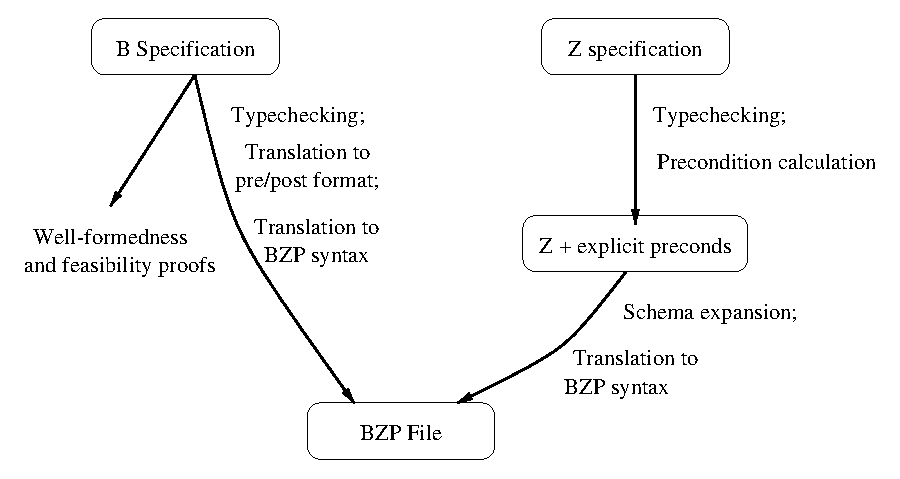
\includegraphics[width=\textwidth]{translation}
  \label{fig:translation}
\end{figure}
\end{slide}



\begin{slide}
\heading{BZP Semantics}

Semantically, a BZP machine = a single B machine (no imports),
where all operations are specified in a standard pre/postcondition format:
\[
    outputs \leftarrow opname(inputs) \defs \\
    \t1 \textbf{PRE}\ Precond(s,inputs) \\
    \t1 \textbf{THEN ANY}\ s',outputs'  \\
    \t2   \textbf{WHERE}\ Postcond(s,s',inputs,outputs') \\
    \t4        \fbox{${}\land Invar(s')$}\leftarrow\hbox{(Z-only)}\\
    \t2   \textbf{THEN}\ outputs,s := outputs',s' \\
    \t2   \textbf{END} \\
    \t1 \textbf{END}
\]
\end{slide}



\begin{slide}
\heading{Z difficulty 1: bindings/records}

\[  
\begin{array}{lcl}
    Schema1 &=& [a,b:\nat | a=3 \land b < 2 ] \also
            &=& \{ \lblot a==3, b==0 \rblot, 
                   \lblot a==3, b==1 \rblot \} \also
\end{array}
\]

\emph{Bindings} are like tuples, but have \emph{named} fields.

Only two operations:
\begin{description}
\item[\qquad Construction:] $\lblot a==Expr_1, b==Expr_2 \rblot$
\item[\qquad Selection:] \qquad $Expr.a$
\end{description}

E.g.:  $\exists x:Schema1 @ x.b > 0$. 
\end{slide}


\begin{slide}
\heading{Z difficulty 1: solutions}
\newcommand{\EG}[2]{\framebox[0.6\textwidth][l]{$#1$}\ 
  \framebox[0.3\textwidth][l]{$\phantom{(}#2$}}

Eg: \EG{x = \lblot a==E_1, b==E_2, c==E_3 \rblot}{x.b}

\begin{description}
\item[0] Translator encodes records as nested pairs.\\
\EG{x = (E_1, (E_2, E_3))}{dom(ran(x))}

\item[1a] Solver extended to handle data terms: $xyz(1,3,\{2,4\})$. \\
\EG{x = xyz(E_1, E_2, E_3)}{xyz\_b(x)} \\
where $xyz\_b : xyz \fun \num$ \\
\phantom{where} $\forall A,B,C @ xyz\_b(xyz(A,B,C)) = B$.

\item[1b] \ldots and solver has a `access $n^{th}$ field' operator.
\EG{x = xyz(E_1, E_2, E_3)}{field(x,2)}

\item[2] Solver handles data terms with named fields:
\EG{x = xyz([a=E_1, b=E_2, c=E_3)}{field(x,b)}
\end{description}
\end{slide}


\begin{slide}
\heading{Z difficulty 2: Free Types}
\[
\begin{array}{lcl}
    Suit   &::=& club | diamond | heart | spade  \also
    Play   &::=& pass
               | play \ldata (1 \upto 13) \cross Suit \rdata \also
    Tree   &::=& empty | node \ldata Tree \cross \num \cross Tree \rdata
\end{array}
\]

Possible Solution:  \quad $play(7,club), \quad node(empty,3,empty).$
\end{slide}



\begin{slide}
\heading{Other Z difficulties}
\begin{description}
\item[Generic Definitions:]

\begin{gendef}[A,B]
    map : (A \fun B) \cross \power A \fun \power B
\where
    map = (\lambda f:A \fun B; s:\power A @ \{e:s @ f~e\})
\end{gendef}

\item[$\mu$ choice operator:] ~\ ~

      $(\mu a:T | P(a))$ returns the unique solution of $P$. \\
      Result is undefined if $P$ has 0 or many solutions.

\[
      x = (\mu D|P)  
      \quad \stackrel{?}{\rightarrow} \quad x \in \{D|P\} \land \#\{D|P\}=1
\]
\end{description}
\end{slide}


\begin{slide}
\heading{The BZP format: Nicolas}
\end{slide}



\begin{slide}
\heading{Traversals and Visitors}

Like compilers, formal methods systems require many
traversals of the specification (its abstract syntax tree).

Example: In Jaza, there are 31 kinds of expressions, 15 kinds of
predicates, 4 kinds of declarations, 8 kinds of schema expressions
and about 10 other kinds of structure.  Total: 68 different types of
nodes in the AST.

With a traditional coding style, each traversal algorithm must
handle each of the node types.
 
Jaza has 10 algorithms that traverse the AST:
\end{slide}
\begin{slide}
{
\ptsize{8}
\begin{tabular}{lrcr}
Purpose         & Result Type   & Useful Cases& Lines of Code \\
\hline
unfold          & ErrorOr ZTerm & 18         & 420 \\%DONE 295 
uniquify        & ZTerm         & 4          & 97  \\%ideal, diff scope rules
substitution    & ZTerm         & 4          & 130 \\%ideal, but Subs arg.
optimisation    & ZTerm         & 10         & 113 \\% DONE 75
evaluation      & ErrorOr ZTerm & most       & 695 \\
\hline
freevars        & VarSet        & 4          & 71  \\
estimate-size   & SetSize       & all exprs  & 66  \\ 
CLPSwrite       & ErrorOr String& all        & 186 \\
CLPStype        & CLPSType      & all exprs  & 98  \\
prettyprint     & Doc           & ALL!       & 600 \\
\hline
Total:          &               &            & 2476 \\
\hline
\end{tabular}
}
\end{slide}

\begin{slide}
\heading{Problems with this Style}

\begin{itemize}
\item Repetitive and verbose code $\implies$ maintenance nightmare.\\
  (it is not easy to extend/change the AST).
\item Each new algorithm is large: 68 methods.
\end{itemize}

In OO languages, further disadvantages are:
\begin{itemize}
\item The algorithm is distributed over many classes.
\item Must change AST classes to add a new algorithm.
\end{itemize}
\end{slide}

\begin{slide}
\heading{The Visitor Design Pattern}

\begin{itemize}
\item Primary purpose: to factor out functionality that can be
  applied to an aggregate hierarchy of "element" objects.
  \\
  \textbf{A regression to functional decomposition.}
\item New algorithms can easily be added to the AST just
  by creating a new Visitor subclass.  The algorithm is all
  in that one class.
\item The algorithm need override only a few methods $\implies$ shorter.
\item Essentially: Visitor implements "double dispatch".
  Every AST class (eg. FuncCall) implements 
  \texttt{accept(Visitor v)}, which calls
  \texttt{v.visitFuncCall(this)}.
\item \textbf{Limitation:} handles AST evolution badly, because
  each visitor has a method for every AST node.
  \\
  AST change $\implies$ all visitors must change.
\end{itemize}
\end{slide}

\begin{slide}
\heading{Visitor Examples from Zeta}

The Visitor class has a method $visit(XYZ\ x)$ for each AST class XYZ.
These methods return either null (meaning no change), or a 
rewritten term. The default implementations of these methods
visit all the subterms of the current node, and reconstruct the 
term if any subterms have been changed.

Example: a visitor which substitutes variables in expressions: 
\begin{small}
\begin{verbatim}
class Substitutor extends TermVisitor {
  Map<Name,Expr> theSubs;
  Expr visit(Expr.Variable var){
    if (theSubs.defines(var.name.name))
      return subs.get(var.name.name);
    else 
      return super.visit(var); // DEFAULT(substitute in subterms)
  }
}
\end{verbatim} 
\end{small}

Example 2: A visitor which just reads information.
\begin{small}
\begin{verbatim}
class FreeVarSampler extends TermVisitor {
  Set<Name> free,bounded; // free/bound variables
  Expr visit(Expr.Variable var){
    if (!bounded.contains(var.name.name))
      free = free.include(var.name.name);
    return null; 
  }
  Expr visit(Expr.Quantor quant){
    visit(quant.matrix);
    Set<Name> savedBounded = bounded;
    bounded = bounded.includeAll(declaredVariables(quant.matrix));
    visit(quant.range);
    bounded = savedBounded;
    return null;
  }
  Expr visit(Predicate.Quantor quant){ ... }  }
\end{verbatim}
\end{small}
\end{slide}

\begin{slide}
\heading{Visitor Design Pattern in Haskell?}

Haskell is a lazy functional language, like ML/CAML,
but with `type classes'.  It is not object-oriented and
has no dynamic binding.

Terminology: $value \in type \in class$.\\
\begin{center}
\begin{tabular}{|l|l|}
  \hline
  Haskell                 & Java \\
  \hline
  [type] class            & interface \\
  instance / type         & class \\
  value                   & object \\
  \hline
\end{tabular}
\end{center}

\begin{small}
\begin{verbatim}
class  (Eq a, Show a) => Num a  where
    (+), (-), (*)    :: a -> a -> a
    negate           :: a -> a
    abs, signum      :: a -> a
    fromInteger      :: Integer -> a
\end{verbatim}
\end{small}
\end{slide}


\begin{slide}
\heading{Visitor Design Pattern in Haskell?}
{
\ptsize{8}
\begin{verbatim}
class (Monad m) => Visitor m where
    visitExpr      :: ZExpr -> m ZExpr   -- we have 7 visitXYZ
    visitPred      :: ZPred -> m ZPred   -- methods in total.

    -- Methods for manipulating the environment,
    lookupLocal  :: ZVar -> m ZExpr  -- lookup locals only
    lookupGlobal :: ZVar -> m ZExpr  -- lookup globals only
    -- methods for pushing local variables.
    pushLocal   :: ZVar -> ZExpr -> m ()

    ----------------- Default Implementations --------------------
    -- The default visitors just recurse through the term
    -- Visitor instances will override some cases of these, like this:
    --    myvisitExpr (ZVar v) = ...             (special processing)
    --    myvisitExpr e        = traverseExpr e  (handle all other cases)
    visitExpr = traverseExpr
    visitPred = traversePred
    ... 
\end{verbatim}
}
\end{slide}

\begin{slide}
\ptsize{8}
The default code uses only the Visitor interface,
so works on any instance of it.

\begin{verbatim}
traversePred :: Visitor a => ZPred -> a ZPred
traversePred (ZAnd p q) =
    do  p2 <- visitPred p
        q2 <- visitPred q
        return (ZAnd p2 q2)
\end{verbatim}

In the OptVisitor instance (optimises predicates for execution):
\ptsize{8}
\begin{verbatim}
newtype OptVisitor a = OptVisitor{unWrapOptV :: Env -> (Env,a)}
instance Visitor OptVisitor where
    visitPred = optPredM
    visitBinder = optGfsM
    setEnv e  = OptVisitor (\ _ -> (e,()))
    currEnv   = OptVisitor (\ env -> (env,env))

optPredM :: ZPred -> OptVisitor ZPred
optPredM (ZAnd p q) =
    do  p2 <- visitPred p
        q2 <- visitPred q
        return (opt_zand p2 q2)
optPredM p = traversePred p  -- handles other cases
\end{verbatim}
\end{slide}

\begin{slide}
\heading{Conclusions}

Two Jaza traversals coded in this style so far:
{\ptsize{8}
\begin{tabular}{lrcrr}
Purpose         & Result Type   & Useful Cases& LOC(Trad) & LOC(Visit)\\
\hline
unfold          & ErrorOr ZTerm & 18         & 420  & 295 \\%DONE 295 
uniquify        & ZTerm         & 4          & 97   &\\%ideal, diff scope rules
substitution    & ZTerm         & 4          & 130  &\\%ideal, but Subs arg.
optimisation    & ZTerm         & 10         & 113  & 75 \\% DONE 75
evaluation      & ErrorOr ZTerm & most       & 695 \\
\hline
freevars        & VarSet        & 4          & 71  \\
estimate-size   & SetSize       & all exprs  & 66  \\ 
CLPSwrite       & ErrorOr String& all        & 186 \\
CLPStype        & CLPSType      & all exprs  & 98  \\
prettyprint     & Doc           & ALL!       & 600 \\
\hline
Total:          &               &            & 2476 \\
\hline
\end{tabular}
}
Most important: more maintainable, easier to add new traversals.
\end{slide}
\end{document}
%% END semsamp2.tex
